\documentclass[a4paper]{article} 
\addtolength{\hoffset}{-2.25cm}
\addtolength{\textwidth}{4.5cm}
\addtolength{\voffset}{-3.25cm}
\addtolength{\textheight}{5cm}
\setlength{\parskip}{0pt}
\setlength{\parindent}{0in}

\usepackage{charter}
\usepackage[utf8]{inputenc}
\usepackage{microtype}
\usepackage[english]{babel}
\usepackage{amsthm, amsmath, amssymb}
\usepackage{float}
\usepackage[final, colorlinks = true, 
            linkcolor = black, 
            citecolor = black]{hyperref}
\usepackage{graphicx, multicol}
\usepackage{xcolor}
\usepackage{marvosym, wasysym}
\usepackage{rotating}
\usepackage{censor}
\usepackage{listings, style/lstlisting}
\usepackage{pseudocode}
\usepackage{style/avm} 
\usepackage{booktabs}
\usepackage[backend=biber,style=numeric,
            sorting=nyt]{biblatex}
\addbibresource{references.bib}
\usepackage{csquotes}
\usepackage[yyyymmdd]{datetime}
\renewcommand{\dateseparator}{-}

\usepackage{fancyhdr} 
\pagestyle{fancy} 
\fancyhead{}\renewcommand{\headrulewidth}{0pt}
\fancyfoot[L]{Udacity Machine Learning Engineer Nanodegree}
\fancyfoot[C]{}
\fancyfoot[R]{\thepage}

\newcommand{\note}[1]{\marginpar{\scriptsize \textcolor{red}{#1}}}

\begin{document}
\title{template_assignment (ECL)}
\fancyhead[C]{}
\hrule \medskip 
\begin{minipage}{0.295\textwidth}
\raggedright
Udacity\\ 
\footnotesize 
\hfill\\
Luiz Alberto Ferreira Gomes
\end{minipage}
\begin{minipage}{0.4\textwidth} 
\centering 
\large 
Capstone Proposal\\ 
\normalsize 
Machine Learning Engineer Nanodegree\\ 
\end{minipage}
\begin{minipage}{0.295\textwidth} 
\raggedleft
\today\\ 
\footnotesize 
\hfill\\
gomes.luiz@gmail.com 
\end{minipage}
\medskip\hrule 
\bigskip

%\begin{multicols}{2}
%[
\section{Project Overview}
Bug Report Tracking Systems(BTS), such as Bugzilla or Jira, have played a major role in the maintenance process in many software development settings, both in Closed Source Software (CSS) and in Open Source Software (OSS). This fact is especially true in OSS projects -- characterized by many users and developers with different levels of expertise spread out the world -- who might create or be responsible for dealing with several bug reports. A user interacts with a BTS often through a simple mechanism called bug report form\cite{Tian:2012}. This kind of form enables users to request changes, to report bugs, or to ask for support in a software product. Initially, he or she should inform a short description, a long description, a type (e.g., bug, new feature, improvement, and task), and an associated severity level (e.g., blocker, critical, major, minor, and trivial). Subsequently, a development team member will review this request and, in case it is not refused for some reason (e.g., bug report duplication), he or she will complete the information in bug report form, indicating, for example, its severity and assigning the person responsible for the bug report. \cite{Cavalcanti:2014}. In this context, my project proposes a machine learning web application for bug severity prediction based on the bug description filled by users when they open a bug in a BTS.

\subsection{Problem Statement}
The severity level information is recognized as a critical variable in the equation to estimate a prioritization of bugs. It defines how soon the bug report needs to be addressed. However, the severity level assignment remains mostly a manual process that relies only on the experience and expertise of the person who has opened the bug report~\cite{Yang:2017}. As a consequence, it is a process with a high degree of subjectivity, and it may be quite error-prone. The number of bug reports in large and medium software OSS projects is frequently very large. Severity level shifts throughout the bug report lifecycle may harm the planning of maintenance activities. For example, the maintenance team could be assigned to address less significant bug reports before the most important ones.

\bigskip

\section{Solution Statement}
The general purpose of my project is to develop an intelligent ML-based web assistant to help developers and maintenance team to predict the severity level of a bug (blocker, critical, major, minor, or trivial). To meet the goal, the tasks that should be executed are the following:
\begin{enumerate}
    \item Collect bug reports data from a Bugzilla BTS;
    \item Pre-process the description text using text mining techniques (e.g. tokenization).
    \item Train and test a machine learning classifier to predict bug severity level based on bug report description;
    \item Build and deploy a web application to extract a bug report description from a Bugzilla BTS and predict the bug severity level.
\end{enumerate}
%]
\subsection{Datasets and Inputs}
I'll use a dataset with 2395 bug reports, collected from Mozilla project, and available in project GitHub repository\footnote{}, to train and test the predicting model. The Mozilla project encompasses several open-source projects, such as Firefox, Thunderbird, and Bugzilla. Furthermore, it is well-established, has a considerable number of registered bug reports, uses standard repositories, and were being studied in academic research~\cite{Lamkanfi:2010, Lamkanfi:2011, Tian:2012}. Table~\ref{tab:features_descriptions} describes the features of the dataset that will used for bug report severity prediction. Each feature in this table has a description, a category.

\begin{table}[ht!]
    \centering
    \begin{tabular}{@{}p{.20\textwidth}p{.30\textwidth}p{.15\textwidth}p{.10\textwidth}@{}}
    \toprule
    {\bf Feature} & {\bf Description} & {\bf Category} & {\bf Target Label}\\
    \midrule
    Bug id                       & Bug report identifier.  & Quantitative Discrete & No\\
    \midrule
    Description                  & Textual content appearing in the description field of the bug report.                                                                               & Unstructured Text & No\\
    \midrule
    Severity                     & Indicates how severe the problem is – from blocker (``application unusable”) to trivial (``minor cosmetic issue”).                                & Qualitative Ordinal & Yes\\
    \bottomrule 
    \end{tabular}
    \caption{The features and its descriptions of dataset used for bug severity prediction. The target label of prediction model is the {\bf Severity} feature }\\
    \label{tab:features_descriptions}
\end{table}

\bigskip
Figure~\ref{fig:severity_class_distribution} shows the label distribution in the Mozilla dataset, which will be used to train and test the prediction model. As one can observe, the label distribution in the dataset is unbalanced. I'll try some techniques to handle this problem, for instance, class weighting\cite{procrastinator:2021}. 
\begin{figure}[ht!]
    \centering
    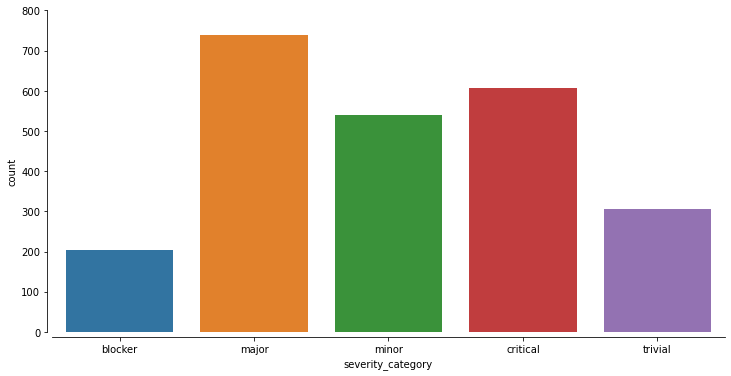
\includegraphics[width=0.8\textwidth]{figures/severity-labels-distribution.png}
    \caption{Caption}
    \label{fig:severity_class_distribution}
\end{figure}

\subsection{Evaluation Metrics}
The specific metrics I'll use for assessing prediction performance for evaluating the accuracy of classification algorithms will be precision, recall, and F-measure, described as follows\cite{Kuhn:2013}:

\begin{itemize}
\item \textbf{Recall}. The recall is the number of True Positives (TP) divided by the number of True Positives (TP) and of False Negatives (FN), where the TP and FN values are derived from the confusion matrix. A low recall indicates many false negatives.

\item \textbf{Precision}. Precision is the number of True Positives (TP) divided by the number of True Positives and False Positives (FP). A low precision can also indicate many false positives.

\item \textbf{F-measure}. F-measure conveys the balance between precision and recall and can be calculated as their harmonic mean. 
\end{itemize}

The metrics above especially useful when the target classes are imbalanced, which often happens in many settings, such as bug severity prediction. Also, these metrics enable the comparison between my prediction model and benchmark models.

\subsection{Benchmarch model}



\section{Project Design}
Figure~\ref{fig:application-architecture} shows the high-level architecture of the bug severity predictor application. The architecture will consist of two modules: front-end and back-end modules. The front-end module will run in a web browser, and it will be in charge of receiving and displaying data from or to the user. The back-end module will run in a server and be responsible for cleaning, breaking into tokens, and weighting each term of the bug description text extracted from a BTS system. Moreover, the back-end module will predict the bug severity level, as requested of the front-end, based on the bug description and the predicting model previously saved. The front-end module will communicate with the back-end throughout the REST protocol. 
\begin{figure}[h!]
    \centering
    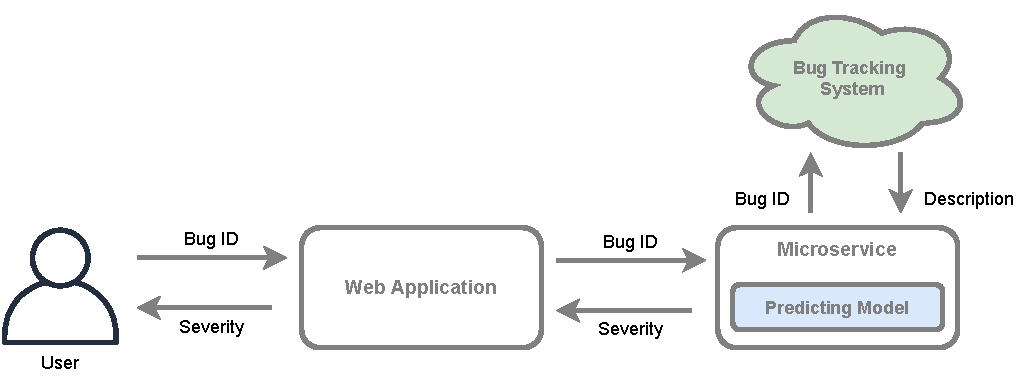
\includegraphics[width=0.8\textwidth]{udacity-capstone-project.pdf}
    \caption{High-level architectural design.}
    \label{fig:application-architecture}
\end{figure}

The predicting model will be train and test using feature extracted using the Pre-training of Deep Bidirectional Transformers for
Language Understanding (BERT)\cite{devlin:2019}.  

\printbibliography

%----------------------------------------------------------------------------------------

\end{document}
